\documentclass[a4paper,11pt]{report}

% You can add margin options here, i.e. [hmargin=3cm,vmargin=4cm]
\usepackage{geometry}

% Select Times New Roman, Helvetica and Courier fonts.
%\usepackage{mathptmx}
%\usepackage[scaled=0.91]{helvet}
%\usepackage{courier}

\usepackage[color,fancy,relax,floatcontrol]{composestar}

% Allows for fixme notes.
% Replace option draft with final when done,
% this will remove the listoffixmes and complain if there are any
% fixmes left in the document.
\usepackage[draft]{fixme}

% Number style 
\usepackage[numbers,sort]{natbib}

% Author, Year style
%\usepackage[authoryear,square]{natbib}
%\let\cite=\citep

% Lay-out of bibliography
\bibliographystyle{abbrvnat}

%\usepackage[Sonny]{fncychap}

% Create evenly spaced table cells.
%\usepackage{tabls}

% Always include hyperref last.
\usepackage[colorlinks=true,bookmarksnumbered,linktocpage,plainpages=false]{hyperref}
% Optionally set the target ancher for hyperref at the top of a figure or table.
% This only works if the figure or table contains a caption.
%\usepackage[figure,table]{hypcap}

% Turn color links black
\hypersetup{%
  linkcolor=black,%
  citecolor=black,%
  pagecolor=black,%
  anchorcolor=black,%
  urlcolor=black%
}

% To include only those chapters I'm currently working on.
%\includeonly{problem,events}

% Make \autoref use the capitalized version just like figure,
% let subsection be the same as section and
% let subfigure be the same as figure.
\renewcommand{\chapterautorefname}{Chapter}
\renewcommand{\sectionautorefname}{Section}
\renewcommand{\subsectionautorefname}{\sectionautorefname}
\newcommand{\subfigureautorefname}{\figureautorefname}

\makenomenclature

% Only show up to level 3 in table of contents.
%\setcounter{tocdepth}{3}
% Show subfloats in list of figures.
%\setcounter{lofdepth}{2}
% Show subfloats in list of listings.
%\setcounter{loldepth}{2}

% Set the graphics path so we just need to add the name and not
% the complete path.
\graphicspath{{./}{./AOSD/images/}{./Composestar/images/}{./DotNET/images/}}

\begin{document}

% Frontmatter.
\title{Some title in \Compose*{}}
\author{Your name goes here}

% Workaround for resetting page count.
% Otherwise a warning is generated (destination with same identifier).
% The page number is suppressed on the title page anyway.
\pagenumbering{alph}
\maketitle

\clearpage
\pagenumbering{roman}% Roman numbering i, ii, ..

%\include{abstract}
%\include{acknowledgements}

\listoffixmes
\tableofcontents
\listoffigures
\lstlistoflistings
\printnomenclature[1in]

\clearpage
\pagenumbering{arabic}% Arabic numbering 1, 2, ..

% Mainmatter
\chapter{Introduction to AOSD}
\label{chp:AOSD}

The first two chapters have originally been written by seven \MSc students~\cite{Holljen2004, Durr2004, Vinkes2004, Bosman2004, Staijen2005, Havinga2005, Boschman2006} at the University of Twente.
The chapters have been rewritten for use in the following theses~\cite{VanOudheusden2006, Conradi2006, TeWinkel2006, Huttenhuis2006, Doornenbal2006, Huisman2006, SpenkelinkD2006}.
They serve as a general introduction into Aspect-Oriented Software Development and \Compose* in particular.

\section{Introduction}
\nomenclature{AOP}{Aspect-Oriented Programming}%
\nomenclature{OOP}{Object-Oriented Programming}%

\begin{figure}
  \centering
  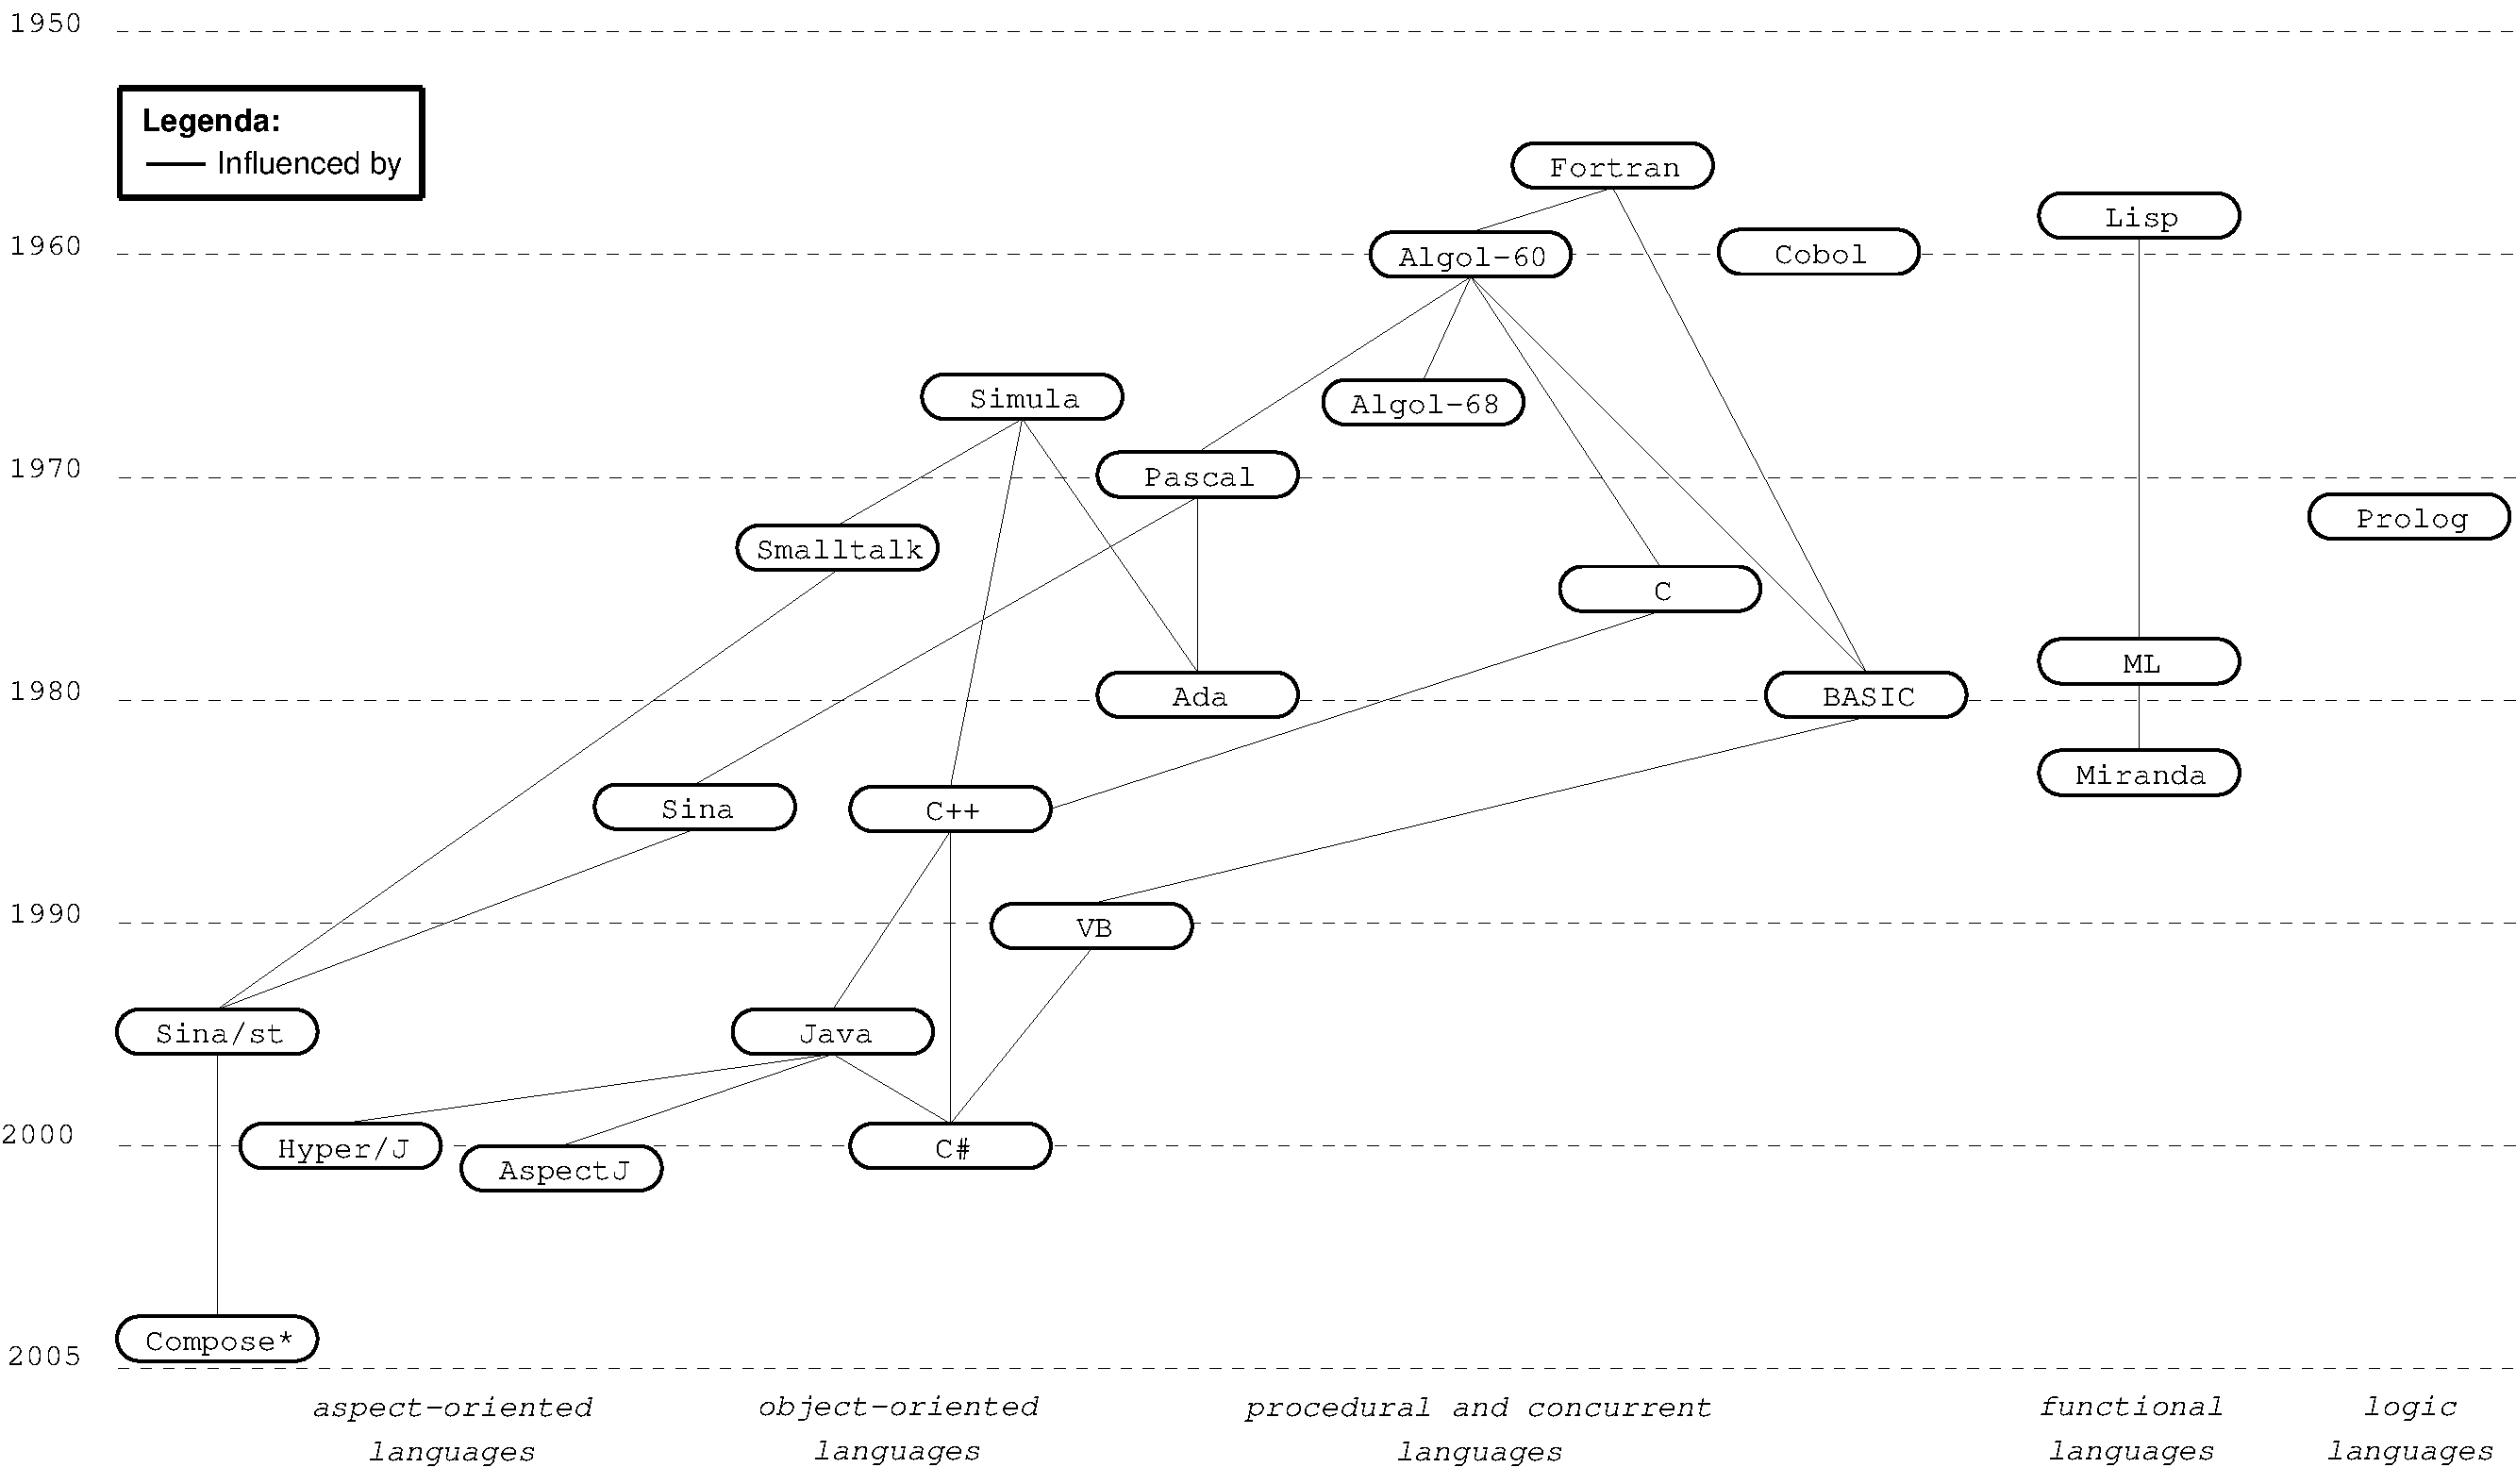
\includegraphics[style=thirdheight]{programming_languages}
  \caption{Dates and ancestry of several important languages}
  \label{fig:programming_languages}
\end{figure}

The goal of software engineering is to solve a problem by implementing a software system.
The things of interest are called concerns.
They exist at every level of the engineering process.
A recurrent theme in engineering is that of modularization: separation and localization of concerns.
The goal of modularization is to create maintainable and reusable software.
A programming language is used to implement concerns.

Fifteen years ago the dominant programming language paradigm was procedural programming.
This paradigm is characterized by the use of statements that update state variables.
Examples are Algol-like languages such as Pascal, C, and Fortran.

Other programming paradigms are the functional, logic, object-oriented, and aspect-oriented paradigms.
\autoref{fig:programming_languages} summarizes the dates and ancestry of several important languages~\cite{Watt90}.
Every paradigm uses a different modularization mechanism for separating concerns into modules.

Functional languages try to solve problems without resorting to variables.
These languages are entirely based on functions over lists and trees.
Lisp and Miranda are examples of functional languages.

A logic language is based on a subset of mathematical logic.
The computer is programmed to infer relationships between values, rather than to compute output values from input values.
Prolog is currently the most used logic language~\cite{Watt90}.

A shortcoming of procedural programming is that global variables can potentially be accessed and updated by any part of the program.
This can result in unmanageable programs because no module that accesses a global variable can be understood independently from other modules that also access that global variable.

The Object-Oriented Programming (OOP) paradigm improves modularity by encapsulating data with methods inside objects.
The data may only be accessed indirectly, by calling the associated methods.
Although the concept appeared in the seventies, it took twenty years to become popular~\cite{Watt90}.
The most well known object-oriented languages are C++, Java, C\#, and Smalltalk.

The hard part about object-oriented design is decomposing a system into objects.
The task is difficult because many factors come into play: encapsulation, granularity, dependency, adaptability, reusability, and others.
They all influence the decomposition, often in conflicting ways~\cite{Gamma95}.

Existing modularization mechanisms typically support only a small set of decompositions and usually only a single dominant modularization at a time.
This is known as the tyranny of the dominant decomposition~\cite{tarr:aosdbook05}.
A specific decomposition limits the ability to implement other concerns in a modular way.
For example, OOP modularizes concerns in classes and only fixed relations are possible.
Implementing a concern in a class might prevent another concern from being implemented as a class.

Aspect-Oriented Programming (AOP) is a paradigm that solves this problem.

AOP is commonly used in combination with OOP but can be applied to other paradigms as well.
The following sections introduce an example to demonstrate the problems that may arise with OOP and show how AOP can solve this.
Finally, we look at three particular AOP methodologies in more detail.

\section{Traditional Approach}

Consider an application containing an object \lstinline|Add| and an object \lstinline|CalcDisplay|.
\lstinline|Add| inherits from the abstract class \lstinline|Calculation| and implements its method \lstinline|execute(a, b)|. 
It performs the addition of two integers.
\lstinline|CalcDisplay| receives an update from \lstinline|Add| if a calculation is finished and prints the result to screen.
Suppose all method calls need to be traced.
The objects use a \lstinline|Tracer| object to write messages about the program execution to screen.
This is implemented by a method called \lstinline|write|.
Three concerns can be recognized: addition, display, and tracing.
The implementation might look something like \autoref{lst:calc_no_aspects}.

\begin{lstsub}
\begin{adjustwidth}{-2cm}{-2cm}%
\centering
\begin{lstsublisting}[style=listing,language=Java,escapeinside={&$}{$&},%
                      caption={Addition},label={lst:calc_no_aspects_add}]{8cm}
public class Add extends Calculation{

  private int result;
  private CalcDisplay calcDisplay;
  private Tracer trace;&$\label{line:cc_1}$&

  Add() {
    result = 0;
    calcDisplay = new CalcDisplay();
    trace = new Tracer();&$\label{line:cc_2}$&
  }

  public void execute(int a, int b) {
    trace.write("void Add.execute(int, int)");&$\label{line:cc_3}$&
    result = a + b;
    calcDisplay.update(result);
  }

  public int getLastResult() {
    trace.write("int Add.getLastResult()");&$\label{line:cc_4}$&
    return result;
  }
}
\end{lstsublisting}\qquad
\begin{lstsublisting}[style=listing,language=Java,escapeinside={&$}{$&},%
                      caption={CalcDisplay},label={lst:calc_no_aspects_calcdisplay}]{8cm}
public class CalcDisplay {
  private Tracer trace;&$\label{line:cc_5}$&

  public CalcDisplay() {
    trace = new Tracer();&$\label{line:cc_6}$&
  }

  public void update(int value){
    trace.write("void CalcDisplay.update(int)");&$\label{line:cc_7}$&
    System.out.println("Printing new value of calculation: "+value);
  }
}
\end{lstsublisting}%
\end{adjustwidth}%
\caption{Modeling addition, display, and logging without using aspects}%
\label{lst:calc_no_aspects}%
\end{lstsub}

From our example, we recognize two forms of crosscutting: \emph{code tangling} and \emph{code scattering}.

The addition and display concerns are implemented in classes \lstinline|Add| and \lstinline|CalcDisplay| respectively.
Tracing is implemented in the class \lstinline|Tracer|, but also contains code in the other two classes (lines~\ref{line:cc_1}, \ref{line:cc_2}, \ref{line:cc_3}, and \ref{line:cc_4} in (a) and \ref{line:cc_5}, \ref{line:cc_6}, and \ref{line:cc_7} in (b)).
If a concern is implemented across several classes it is said to be scattered.
In the example of \autoref{lst:calc_no_aspects} the tracing concern is scattered.

Usually a scattered concern involves code \emph{replication}.
That is, the same code is implemented a number of times.
In our example the classes \lstinline|Add| and \lstinline|CalcDisplay| contain similar tracing code.

In class \lstinline|Add| the code for the addition and tracing concerns are intermixed.
In class \lstinline|CalcDisplay| the code for the display and tracing concerns are intermixed.
If more then one concern is implemented in a single class they are said to be tangled.
In our example the addition and tracing concerns are tangled.
Also display and tracing concerns are tangled.
Crosscutting code has the following consequences:
\begin{description}[style=nextline,noitemsep]
  \item[Code is difficult to change] Changing a scattered concern requires us to modify the code in several places.
Making modifications to a tangled concern class requires checking for side-effects with all existing crosscutting concerns;
  \item[Code is harder to reuse] To reuse an object in another system, it is necessary to either remove the tracing code or reuse the (same) tracer object in the new system;
  \item[Code is harder to understand] Tangled code makes it difficult to see which code belongs to which concern.
\end{description}

\section{AOP Approach}

To solve the problems with crosscutting, several techniques are being researched that attempt to increase the expressiveness of the OO paradigm.
Aspect-Oriented Programming (AOP) introduces a modular structure, the aspect, to capture the location and behavior of crosscutting concerns.
Examples of Aspect-Oriented languages are Sina, AspectJ, Hyper/J, and \Compose*.
A special syntax is used to specify aspects and the way in which they are combined with regular objects.
The fundamental goals of AOP are twofold~\cite{gradecki:maj03}: first to provide a mechanism to express concerns that crosscut other components.
Second to use this description to allow for the separation of concerns.

\emph{Join points} are well-defined places in the structure or execution flow of a program where additional behavior can be attached.
The most common join points are method calls.
\emph{Pointcuts} describe a set of join points.
This allows us to execute behavior at many places in a program by one expression.
\emph{Advice} is the behavior executed at a join point.

In the example of \autoref{lst:calc_aspects} the class \lstinline|Add| does not contain any tracing code and only implements the addition concern.
Class \lstinline|CalcDisplay| also does not contain tracing code.
In our example the tracing aspect contains all the tracing code.
The pointcut \lstinline|tracedCalls| specifies at which locations tracing code is executed.

\begin{lstsub}
\begin{adjustwidth}{-2cm}{-2cm}%
\centering
\begin{lstsublisting}[style=listing,language=Java,%
                      caption={Addition concern},label={lst:calc_base_add}]{75mm}
public class Add extends Calculation{
  private int result;
  private CalcDisplay calcDisplay;

  Add() {
    result = 0;
    calcDisplay = new CalcDisplay();
  }

  public void execute(int a, int b) {
    result = a + b;
    calcDisplay.update(result);
  }

  public int getLastResult() {
  	return result;
  }
}
\end{lstsublisting}\qquad
\begin{lstsublisting}[style=listing,language={[AspectJ]Java},%
                      caption={Tracing concern},label={lst:calc_trace_concern}]{85mm}
aspect Tracing {
  Tracer trace = new Tracer();

  pointcut tracedCalls(): 	 
    call(* (Calculation+).*(..)) ||
    call(* CalcDisplay.*(..));

  before(): tracedCalls() {
    trace.write(thisJoinPoint.getSignature().toString());
  }
}\end{lstsublisting}%
\end{adjustwidth}%
\caption{Modeling addition, display, and logging with aspects}%
\label{lst:calc_aspects}%
\end{lstsub}

The crosscutting concern is explicitly captured in aspects instead of being embedded within the code of other objects.
This has several advantages over the previous code.
\begin{description}[style=nextline,noitemsep]
  \item[Aspect code can be changed] Changing aspect code does not influence other concerns;
  \item[Aspect code can be reused] The coupling of aspects is done by defining pointcuts. In theory, this low coupling allows for reuse. In practice reuse is still difficult;
  \item[Aspect code is easier to understand] A concern can be understood independent of other concerns;
  \item[Aspect pluggability] Enabling or disabling concerns becomes possible.
\end{description}

\subsection{AOP Composition}
\label{sec:AOPComposition}

AOP composition can be either symmetric or asymmetric.
In the symmetric approach every component can be composed with any other component.
This approach is followed by e.g. Hyper/J.

In the asymmetric approach, the base program and aspects are distinguished.
The base program is composed with the aspects.
This approach is followed by e.g. AspectJ (covered in more detail in the next section).

\subsection{Aspect Weaving}
\label{sec:AspectWeaving}

\nomenclature{IL}{Intermediate Language}%
\nomenclature{CIL}{Common Intermediate Language}%
The integration of components and aspects is called \emph{aspect weaving}.
There are three approaches to aspect weaving.
The first and second approach rely on adding behavior in the program, either by weaving the aspect in the source code, or by weaving directly in the target language.
The target language can be intermediate language (IL) or machine code.
Examples of IL are Java byte code and Common Intermediate Language (CIL).
The remainder of this chapter considers only intermediate language targets.
The third approach relies on adapting the virtual machine.
Each method is explained briefly in the following sections.

\subsubsection{Source Code Weaving}
\label{sec:source_code_weaving}

The source code weaver combines the original source with aspect code.
It interprets the defined aspects and combines them with the original source, generating input for the native compiler.
For the native compiler there is no difference between source code with and without aspects.
Hereafter the compiler generates an intermediate or machine language output (depending on the compiler-type).

The advantages of using source code weaving are:
\begin{description}[style=nextline,noitemsep]
  \item[High-level source modification] Since all modifications are done at source code level, there is no need to know the target (output) language of the native compiler;
  \item[Aspect and original source optimization] First the aspects are woven into the source code and hereafter compiled by the native compiler.
       The produced target language has all the benefits of the native compiler optimization passes.
       However, optimizations specific to exploiting aspect knowledge are not possible;
  \item[Native compiler portability] The native compiler can be replaced by any other compiler as long as it has the same input language.
       Replacing the compiler with a newer version or another target language can be done with little or no modification to the aspect weaver.
\end{description}

However, the drawbacks of source code weaving are:
\begin{description}[style=nextline,noitemsep]
  \item[Language dependency] Source code weaving is written explicitly for the syntax of the input language;
  \item[Limited expressiveness] Aspects are limited to the expressive power of the source language.
       For example, when using source code weaving, it is not possible to add multiple inheritance to a single inheritance language.
\end{description}

\subsubsection{Intermediate Language Weaving}
\label{sec:intermediate_language_weaving}

Weaving aspects through an intermediate language gives more control over the executable program and solves some issues as identified in \autoref{sec:source_code_weaving} on source code weaving.
Weaving at this level allows for creating combinations of intermediate language constructs that can not be expressed at the source code level.
Although IL can be hard to understand, IL weaving has several advantages over source code weaving:
\begin{description}[style=nextline,noitemsep]
  \item[Programming language independence] All compilers generating the target IL output can be used;
  \item[More expressiveness] It is possible to create IL constructs that are not possible in the original programming language;
  \item[Source code independence] Can add aspects to programs and libraries without using the source code (which may not be available);
  \item[Adding aspects at load- or runtime] A special class loader or runtime environment can decide and do dynamic weaving.
       The aspect weaver adds a runtime environment into the program.
       How and when aspects can be added to the program depend on the implementation of the runtime environment.
\end{description}

However, IL weaving also has drawbacks that do not exist for source code weaving:
\begin{description}[style=nextline,noitemsep]
  \item[Hard to understand] Specific knowledge about the IL is needed;
  \item[More error-prone] Compiler optimization may cause unexpected results.
       Compiler can remove code that breaks the attached aspect (\eg inlining of methods).
\end{description}

\subsubsection{Adapting the Virtual Machine}

\nomenclature{VM}{Virtual Machine}%
Adapting the virtual machine (VM) removes the need to weave aspects.
This technique has the same advantages as intermediate language weaving and can also overcome some of its disadvantages as mentioned in \autoref{sec:intermediate_language_weaving}.
Aspects can be added without recompilation, redeployment, and restart of the application~\cite{popovici:aosd02,popovici:aosd03}.

Modifying the virtual machine also has its disadvantages:
\begin{description}[style=nextline,noitemsep]
  \item[Dependency on adapted virtual machines] Using an adapted virtual machine requires that every system should be upgraded to that version;
  \item[Virtual machine optimization] People have spend a lot of time optimizing virtual machines.
       By modifying the virtual machine these optimizations should be revisited.
       Reintegrating changes introduced by newer versions of the original virtual machine, might have substantial impact.
\end{description}


\section{AOP Solutions}
\label{sec:AOPSolutions}

As the concept of AOP has been embraced as a useful extension to classic programming, different AOP solutions have been developed.
Each solution has one or more implementations to demonstrate how the solution is to be used. 
As described by~\cite{elrad:cacm01} these differ primarily in:
\begin{description}[style=nextline,noitemsep]
  \item[How aspects are specified] Each technique uses its own aspect language to describe the concerns;
  \item[Composition mechanism] Each technique provides its own composition mechanisms;
  \item[Implementation mechanism] Whether components are determined statically at compile time or dynamically at run time, the support for verification of compositions, and the type of weaving.
  \item[Use of decoupling] Should the writer of the main code be aware that aspects are applied to his code;
  \item[Supported software processes] The overall process, techniques for reusability, analyzing aspect performance of aspects, is it possible to monitor performance, and is it possible to debug the aspects.
\end{description}

This section will give a short introduction to AspectJ~\cite{kiczales:ecoop01} and Hyperspaces~\cite{ossher:sact01}, which together with Composition Filters~\cite{bergmans:cacm01} are three main AOP approaches.

\subsection{AspectJ Approach}
\label{sec:TheAspectJApproach}

\emph{AspectJ}~\cite{kiczales:ecoop01} is an aspect-oriented extension to the Java programming language.
It is probably the most popular approach to AOP at the moment, and it is finding its way into the industrial software development.
AspectJ has been developed by Gregor Kiczales at Xerox's PARC (Palo Alto Research Center).
To encourage the growth of the AspectJ technology and community, PARC transferred AspectJ to an open Eclipse project.
The popularity of AspectJ comes partly from the various extensions based on it, build by several research groups.
There are various projects that are porting AspectJ to other languages, resulting in tools such as AspectR and AspectC.

One of the main goals in the design of AspectJ is to make it a compatible extension to Java.
AspectJ tries to be compatible in four ways:
\begin{description}[style=nextline,noitemsep]
  \item[Upward compatibility] All legal Java programs must be legal AspectJ programs;
  \item[Platform compatibility] All legal AspectJ programs must run on standard Java virtual machines;
  \item[Tool compatibility] It must be possible to extend existing tools to support AspectJ in a natural way; this includes IDEs, documentation tools and design tools;
  \item[Programmer compatibility] Programming with AspectJ must feel like a natural extension of programming with Java.
\end{description}

AspectJ extends Java with support for two kinds of crosscutting functionality.
The first allows defining additional behavior to run at certain well-defined points in the execution of the program and is called the \emph{dynamic crosscutting mechanism}.
The other is called the \emph{static crosscutting mechanism} and allows modifying the static structure of classes (methods and relationships between classes).
The units of crosscutting implementation are called aspects.
An example of an aspect specified in AspectJ is shown in \autoref{lst:dynamiccrosscuttingexample}.

\begin{lstlisting}[language={[AspectJ]Java},style=floatlisting,%
                   caption={Example of dynamic crosscutting in AspectJ},%
                   label={lst:dynamiccrosscuttingexample}]
aspect DynamicCrosscuttingExample {
  Log log = new Log();

  pointcut traceMethods():
    execution(edu.utwente.trese.*.*(..));

  before() : traceMethods {
    log.write("Entering " + thisJointPoint.getSignature());
  }

  after() : traceMethods {
    log.write("Exiting " + thisJointPoint.getSignature());
  }
}
\end{lstlisting}

The points in the execution of a program where the crosscutting behavior is inserted are called \emph{join points}.
A \emph{pointcut} has a set of join points.
In \autoref{lst:dynamiccrosscuttingexample} is \lstinline|traceMethods| an example of a pointcut definition.
The pointcut includes all executions of any method that is in a class contained by package \lstinline|edu.utwente.trese|.

The code that should execute at a given join point is declared in an advice.
Advice is a method-like code body associated with a certain pointcut.
AspectJ supports \emph{before}, \emph{after} and \emph{around} advice, which specifies where the additional code is to be inserted.
In the example both before and after advice are declared to run at the join points specified by the \lstinline|traceMethods| pointcut.

Aspects can contain anything permitted in class declarations including definitions of pointcuts, advice and static crosscutting.
For example, static crosscutting allows a programmer to add fields and methods to certain classes as shown in \autoref{lst:staticcrosscuttingexample}.

\begin{lstlisting}[language={[AspectJ]Java},style=floatlisting,%
                   caption={Example of static crosscutting in AspectJ},%
                   label={lst:staticcrosscuttingexample},floatplacement=htbp]
aspect StaticCrosscuttingExample {
  private int Log.trace(String traceMsg) {
    Log.write(" --- MARK --- " + traceMsg);
  }
}
\end{lstlisting}

The shown construct is called inter-type member declaration and adds a method \lstinline|trace| to class \lstinline|Log|.
Other forms of inter-type declarations allow developers to declare the parents of classes (super classes and realized interfaces), declare where exceptions need to be thrown, and allow a developer to define the precedence among aspects.

With its variety of possibilities, AspectJ can be considered a useful approach for realizing software requirements.

\subsection{Hyperspaces Approach}

The \emph{Hyperspaces} approach is developed by H.~Ossher and P.~Tarr at the IBM T.J.~Watson Research Center.
The Hyperspaces approach adopts the principle of multi-dimensional separation of concerns~\cite{ossher:sact01}, which involves:
\begin{itemize}[noitemsep]
  \item Multiple, arbitrary dimensions of concerns;
  \item Simultaneous separation along these dimensions;
  \item Ability to dynamically handle new concerns and new dimensions of concern as they arise throughout the software life cycle;
  \item Overlapping and interacting concerns. It is appealing to think of many concerns as independent or orthogonal, but they rarely are in practice.
\end{itemize}

We explain the Hyperspaces approach by an example written in the \emph{Hyper/J} language.
Hyper/J is an implementation of the Hyperspaces approach for Java.
It provides the ability to identify concerns, specify modules in terms of those concerns, and synthesize systems and components by integrating those modules.
Hyper/J uses byte code weaving on binary Java class files and generates new class files to be used for execution.
Although the Hyper/J project seems abandoned and there has not been any update in the code or documentation for a while, we still mention it because the Hyperspaces approach offers a unique AOP solution.

As a first step, developers create hyperspaces by specifying a set of Java class files that contain the code units that populate the hyperspace.
To do this, you create a hyperspace specification, as demonstrated in \autoref{lst:hyperspaces1}.

\begin{lstlisting}[language={[HyperJ]Java},style=floatlisting,%
                   caption={Creation of a hyperspace},label={lst:hyperspaces1},%
                   floatplacement=htbp]
Hyperspace Pacman
  class edu.utwente.trese.pacman.*;
\end{lstlisting}

Hyper/J will automatically create a hyperspace with one dimension---the class file dimension.
A dimension of concern is a set of concerns that are disjoint.
The initial hyperspace will contain all units within the specified package.
To create a new dimension you can specify concern mappings, which describe how existing units in the hyperspace relate to concerns in that dimension, as demonstrated in \autoref{lst:hyperspaces2}.

\begin{lstlisting}[language={[HyperJ]Java},style=floatlisting,%
                   caption={Specification of concern mappings},label={lst:hyperspaces2},%
                   floatplacement=htbp]
package edu.utwente.trese.pacman: Feature.Kernel
operation trace: Feature.Logging
operation debug: Feature.Debugging
\end{lstlisting}

The first line indicates that, by default, all of the units contained within the package \lstinline|edu.utwente.trese.pacman| address the kernel concern of the feature dimension.
The other mappings specify that any method named \lstinline|trace| or \lstinline|debug| address the logging and debugging concern respectively.
These later mappings override the first one.

Hypermodules are based on concerns and consist of two parts.
The first part specifies a set of hyperslices in terms of the concerns identified in the concern matrix.
The second part specifies the integration relationships between the hyperslices.
A hyperspace can contain several hypermodules realizing different modularizations of the same units.
Systems can be composed in many ways from these hypermodules.

\begin{lstlisting}[language={[HyperJ]Java},style=floatlisting,%
                   caption={Defining a hypermodule},label={lst:hyperspaces3},%
                   floatplacement=htbp]
hypermodule Pacman_Without_Debugging
  hyperslices: Feature.Kernel, Feature.Logging;
  relationships: mergeByName;
end hypermodule;
\end{lstlisting}

\autoref{lst:hyperspaces3} shows a hypermodule with two concerns, kernel and logging.
They are related by a \lstinline|mergeByName| integration relationship.
This means that units in the different concerns correspond if they have the same name (\lstinline|ByName|) and that these corresponding units are to be combined (\lstinline|merge|).
For example, all members of the corresponding classes are brought together into the composed class.
The hypermodule results in a hyperslice that contains all the classes without the debugging feature; thus no \lstinline|debug| methods will be present.

The most important feature of the hyperspaces approach is the support for on-demand remodularisation: the ability to extract hyperslices to encapsulate concerns that were not separated in the original code.
Which makes hyperspaces especially useful for evolution of existing software.

\subsection{Composition Filters}
\label{sec:Composition_Filters}

\nomenclature{CF}{Composition Filters}%
\emph{Composition Filters} is developed by M.~Ak\c{s}it and L.~Bergmans at the TRESE group, which is a part of the Department of Computer Science of the University of Twente, The Netherlands.
The composition filters (CF) model predates aspect-oriented programming.
It started out as an extension to the object-oriented model and evolved into an aspect-oriented model.
The current implementation of CF is \Compose*, which covers \dotNET, Java, and C.

One of the key elements of CF is the \emph{message}, a message is the interaction between objects, for instance a method call.
In object-oriented programming the message is considered an abstract concept. In the implementations of CF it is therefore necessary to reify the message.
This \emph{reified message} contains properties, like where it is send to and where it came from.

The concept of CF is that messages that enter and exit an object can be intercepted and manipulated, modifying the original flow of the message.
To do so, a layer called the \emph{interface part} is introduced in the CF model, this layer can have several properties.
The interface part can be placed on an object, which behavior needs to be altered, and this object is referred to as \emph{inner}.

%\begin{figure}
%  \centering
%  \includegraphics[style=thirdheight]{cfmodel}
%  \caption{Components of the composition filters model}
%  \label{fig:cfmodel}
%\end{figure}

There are three key elements in CF: messages, filters, and superimposition.
Messages are sent from one object to another, if there is an interface part placed on the receiver, then the message that is sent goes through the input filters.
In the filters the message can be manipulated before it reaches the inner part, the message can even be sent to another object.
How the message will be handled depends on the filter type.
An output filter is similar to an input filter, the only difference is that it manipulates messages that originate from the inner part.
The latest addition to CF is superimposition, which is used to specify which interfaces needs to be superimposed on which
inner objects.

%\begin{lstlisting}[language=ComposeStar,style=floatlisting,%
%                   caption={Example of a filter module specification},label={lst:concern}]
%concern interfaceSound in pacman {
%  filtermodule beepSound {
%    internals
%      beeper : pacman.ConcernImplementations.Beeper;
%    conditions
%      soundOff : pacman.Game.isSoundOn();
%    inputfilters
%      soundOff_filter : Dispatch = {soundOff => [*.*] *.*};
%      beep_filter : Meta = {
%        [*.eatFood] beeper.eatBeep,
%        [*.eatGhost] beeper.eatGhostBeep,
%        [*.eatVitamin] beeper.powerBeep,
%        [*.pacmanKilled] beeper.bumpGhostBeep }
%  }
%}
%\end{lstlisting}

%The message manipulation mechanism of the CF model is explained by means of an example demonstrated in \autoref{lst:concern}.
%This example uses a dispatch filter and a meta filter.
%When \lstinline|soundOff| is true, the dispatch filter will leave the message as it is, this implies that the message will leave the filter and thus will not come through to the second filter.
%The second filter is a meta filter, if the message is send to the method \lstinline|eatFood|, then the filter status is send as a message to \lstinline|beeper.eatBeep|.
%If the message does not have \lstinline|eatFood| as selector, the filter tries the other options from right to the left until there is a match. If there is no match at all the message will leave the filter unaltered.

%The latest addition to CF is superimposition, which is used to specify crosscuts.
%Crosscuts are made by combining a filter module with a selection of objects, as shown in \autoref{lst:concern1}.
%In the given example the filter module \lstinline|tracingModule| is superimposed on every instance of the classes \lstinline|Pacman|, \lstinline|Ghost|, and \lstinline|World|.

%\begin{lstlisting}[language=ComposeStar,style=floatlisting,%
%                   caption={Example of the use of superimposition},label={lst:concern1}]
%concern Tracing {
%  filtermodule tracingModule { }
%
%  superimposition {
%    selectors
%      withTracing = { C | isClassWithNameInList(C,
%                          ['Pacman', 'Ghost', 'World']) };
%    filtermodules
%      withTracing <- tracingModule;
%  }
%}
%\end{lstlisting}



\chapter{\Compose*{}}
\begin{flushright}
\textit{The difficult part of composition filters}\\
\textit{is understanding its simplicity.}\\
\textit{Lodewijk Bergmans}\\
\end{flushright}

\label{chp:ComposeStar}

\Compose* is an implementation of the composition filters approach. There are three target environments: the \dotNET, Java, and C.
This chapter is organized as follows, first the evolution of Composition Filters and its implementations are described, followed by an explanation of the \Compose* language and a demonstrating example. 
In the third section, the \Compose* architecture is explained, followed by a description of the features specific to \Compose*.

\section{Evolution of Composition Filters}
\Compose* is the result of many years of research and experimentation.
The following time line gives an overview of what has been done in the years before and during the \Compose* project.

\begin{description}[noitemsep,style=sameline,leftmargin=15mm]
\item[1985] The first version of Sina is developed by Mehmet Ak\c{s}it.
            This version of Sina contains a preliminary version of the composition filters concept called semantic networks.
            The semantic network construction serves as an extension to objects, such as classes, messages, or instances.
            These objects can be configured to form other objects such as classes from which instances can be created.
            The object manager takes care of synchronization and message processing of an object.
            The semantic network construction can express key concepts like delegation, reflection, and synchronization~\cite{koopmans:sina95}.
\item[1987] Together with Anand Tripathi of the University of Minnesota the Sina language is further developed.
            The semantic network approach is replaced by declarative specifications and the interface predicate construct is added.
\item[1991] The interface predicates are replaced by the dispatch filter, and the wait filter manages the synchronization functions of the object manager.
            Message reflection and real-time specifications are handled by the meta filter and the real-time filter~\cite{bergmans:phd94}.
\item[1995] The Sina language with Composition Filters is implemented using Smalltalk~\cite{koopmans:sina95}.
            The implementation supports most of the filter types.
            In the same year, a preprocessor providing C++ with support for Composition Filters is implemented~\cite{glandrup:ms95}.
\item[1999] The composition filters language ComposeJ~\cite{wichman:ms99} is developed and implemented.
            The implementation consists of a preprocessor capable of translating composition filter specifications into the Java language.
\item[2001] ConcernJ is implemented as part of a \MSc thesis~\cite{salinas:ms01}.
            ConcernJ adds the notion of superimposition to Composition Filters.
            This allows for reuse of the filter modules and to facilitate crosscutting concerns.
\item[2003] The start of the \Compose* project, the project is described in further detail in this chapter.
\item[2004] The first release of \Compose*, based on \dotNET.
\item[2005] The start of the Java port of \Compose*.
\item[2006] Porting \Compose* to C is started.
\end{description}

%\section{Composition Filters}
\section{Composition Filters in \Compose*{}}
\label{sec:CompositionFiltersInComposeStar}
% Removed "t" so that it is not longer breaking the history list
\begin{lstlisting}[language=Composestar,style=floatlisting,float=hbp, caption={Abstract concern template},label={lst:concerntemplate}]
concern {
  filtermodule {
    internals
    externals
    conditions
    inputfilters
    outputfilters
  }
  superimposition {
    selectors
    filtermodules
    annotations
    constraints
  }
  implementation
}
\end{lstlisting}
A \Compose* application consists of concerns that can be divided in three parts: filter module specifications, superimposition, and implementation.
A filter module contains the filter logic to filter on incoming or outgoing messages on superimposed objects.
Messages have a target, which is an object reference, and a selector, which is a method name.
A superimposition part specifies which filter modules, annotations, conditions, and methods are superimposed on which objects.
An implementation part contains the class implementation of a concern.
How these parts are placed in a concern is shown in \autoref{lst:concerntemplate}.

\begin{figure}[hbp]
  \centering
  \includegraphics[style=thirdheight]{cfmodel}
  \caption{Components of the composition filters model}
  \label{fig:cfmodel}
\end{figure}

The working of a filter module is depicted in \autoref{fig:cfmodel}.
A filter module can contain input and output filters.
The difference between these two sets of filters is that the first is used to filter on incoming messages, while the second is used to filter on outgoing messages.
The return of a method is not considered an outgoing message.
A filter has three parts: a filter identifier, a filter type, and one or more filter elements.
A filter element exists out of an optional condition part, a matching part, and a substitution part.
These parts are shown below:
\begin{center}
$\overbrace{stalker\_filter}^{identifier}:\overbrace{Dispatch}^{filter~type}~=~\{\overbrace{!pacmanIsEvil}^{condition~part}
=>\overbrace{[*.getNextMove]}^{matching~part}~\overbrace{stalk\_strategy.getNextMove}^{substitution~part}~\}$
\end{center}
A filter identifier is a unique name for a filter in a filter module. 
Filters match when both the condition part and the matching part evaluate to true.
In the demonstrated filter, every message where the selector is \lstinline|getNextMove| matches.
If an asterisk~(\lstinline|*|) is used in the target, every target will match.
When the condition part and the matching part are true, the message is substituted with the values provided in the substitution part.
How these values are substituted, and how the message continues, depends on the type of  filter used.
\newpage
At the moment there are four basic filter types defined in \Compose*.
It is, however, possible to write custom filter types.
\begin{description}[style=sameline,leftmargin=18mm]
  \item[Dispatch] If the message is accepted, it is dispatched to the specified target of the message, otherwise the message continues to the subsequent filter.
    This filter type can only be used for input filters;
  \item[Send] If the message is accepted, it is sent to the specified target of the message, otherwise the message continues to the subsequent filter.
    This filter type can only be used for output filters;
  \item[Error] If the filter rejects the message, it raises an exception, otherwise the message continues to the next filter in the set;
  \item[Meta] If the message is accepted, the message is sent as a parameter of another meta message to an internal or external object, otherwise the message just continues to the next filter.
    The object that receives the meta message can observe and manipulate the message and can re-activate the execution of the message.
\end{description}

The identifier \lstinline|pacmanIsEvil|, used in the condition part, must be declared in the conditions section of a filter module.
Targets that are used in a filter can be declared as internal or external.
An internal is an object that is unique for each instance of a filter module, while an external is an object that is shared between filter modules.

Filter modules are superimposed on classes using filter module binding, which specifies a selection of objects on the one side, and a filter module on the other side.
The selection is specified in a selector definition.
This selector definition uses predicates to select objects, such as \lstinline|isClassWithNameInList|, \hbox{\lstinline|isNamespaceWithName|}, and \lstinline|namespaceHasClass|.
In addition to filter modules, it is possible to bind conditions, methods, and annotations to classes using superimposition.

The last part of the concern is the implementation part, which can be used to define the behavior of a concern.
For a logging concern, for example, we can define specific log functions and use them as internal.



%\section{Demonstrating Example}
\section{Demonstrating Example}
\label{sec:demonstratingexample}

To illustrate the \Compose* toolset, this section introduces a \emph{Pacman} example.
The Pacman game is a classic arcade game in which the user, represented by pacman, moves in a maze to eat vitamins.
Meanwhile, a number of ghosts try to catch and eat pacman.
There are, however, four mega vitamins in the maze that make pacman evil.
In its evil state, pacman can eat ghosts.
A simple list of requirements for the Pacman game is briefly discussed here:
\begin{itemize}[noitemsep]
  \item One live is taken from pacman when eaten by a ghost;
  \item A game should end when pacman has no more lives;
  \item The score of a game should increase when pacman eats a vitamin or a ghost;
  \item A user should be able to use a keyboard to move pacman around the maze;
  \item Ghosts should know whether pacman is evil or not;
  \item Ghosts should know where pacman is located;
  \item Ghosts should hunt or flee from pacman, depending on the state of pacman.
\end{itemize}

\subsection{Initial Object-Oriented Design}

\begin{figure}[p]
  \centering
  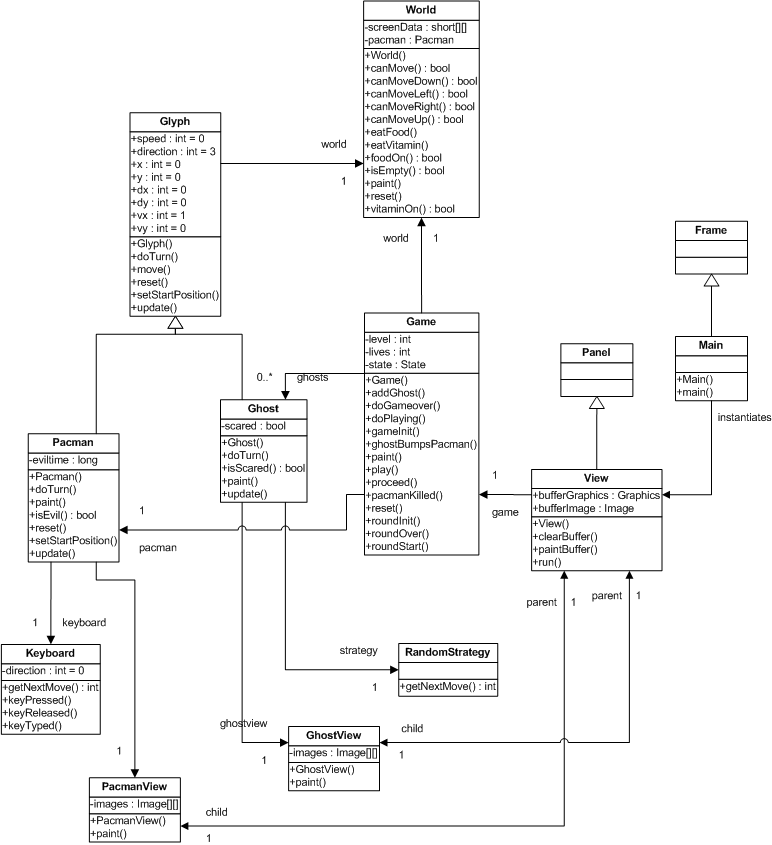
\includegraphics[style=page]{pacman_class_diagram}
  \caption{Class diagram of the object-oriented Pacman game}
  \label{fig:pacman_class_diagram}
\end{figure}
\afterpage{\clearpage}

\nomenclature{UML}{Unified Modeling Language}%
\autoref{fig:pacman_class_diagram} shows an initial object-oriented design for the Pacman game.
Note that this UML class diagram does not show the trivial accessors.
The classes in this diagram are:
%\begin{description}[noitemsep,style=nextline]
\begin{description}[noitemsep,style=sameline,leftmargin=32mm]
  \item [Game] This class encapsulates the control flow and controls the state of a game;
  \item [Ghost] This class is a representation of a ghost chasing pacman.
    Its main attribute is a property that indicates whether it is scared or not (depending on the evil state of pacman);
  \item [GhostView] This class is responsible for painting ghosts;
  \item [Glyph] This is the superclass of all mobile objects (pacman and ghosts).
    It contains common information like direction and speed;
  \item [Keyboard] This class accepts all keyboard input and makes it available to pacman;
  \item [Main] This is the entry point of a game;
  \item [Pacman] This is a representation of the user controlled element in the game.
    Its main attribute is a property that indicates whether pacman is evil or not;
  \item [PacmanView] This class is responsible for painting pacman;
  \item [RandomStrategy] By using this strategy, ghosts move in random directions;
  \item [View] This class is responsible for painting a maze;
  \item [World] This class has all the information about a maze.
    It knows where the vitamins, mega vitamins and most importantly the walls are.
    Every class derived from class \lstinline|Glyph| checks whether movement in the desired direction is possible.
\end{description}

\subsection{Completing the Pacman Example}

The initial object-oriented design, described in the previous section, does not implement all the stated system requirements.
The missing requirements are:
\begin{itemize}[noitemsep]
  \samepage
  \item The application does not maintain a score for the user;
  \item Ghosts move in random directions instead of chasing or fleeing from pacman.
\end{itemize}
In the next sections, we describe why and how to implement these requirements in the \Compose* language.

\subsubsection{Implementation of Scoring}

The first system requirement that we need to add to the existing Pacman game is scoring.
This concern involves a number of events.
First, the score should be set to zero when a game starts.
Second, the score should be updated whenever pacman eats a vitamin, mega vitamin or ghost.
And finally, the score itself has to be painted on the maze canvas to relay it back to the user.
These events scatter over multiple classes: \lstinline|Game| (initializing score), \lstinline|World| (updating score), \lstinline|Main| (painting score).
Thus scoring is an example of a crosscutting concern. 

To implement scoring in the \Compose* language, we divide the implementation into two parts.
The first part is a \Compose* concern definition stating which filter modules to superimpose.
\autoref{lst:scoringconcern} shows an example \Compose* concern definition of scoring.

\begin{lstlisting}[style=listing,escapeinside={&$}{$&},language=ComposeStar,%
                   caption={\expandafter{\lstinline[style=inline]|DynamicScoring|} concern in \Compose*{}},%
                   label={lst:scoringconcern}]
concern DynamicScoring in Pacman {&$\label{line:dynscore_concern}$&
  filtermodule dynamicscoring {&$\label{line:dynscore_fm_begin}$&
    externals
      score : pacman.Score = pacman.Score.instance();
    inputfilters 
      score_filter : Meta = {[*.eatFood] score.eatFood,&$\label{line:score_filter}$&
                             [*.eatGhost] score.eatGhost,
                             [*.eatVitamin] score.eatVitamin,
                             [*.gameInit] score.initScore,
                             [*.setForeground] score.setupLabel}
  }&$\label{line:dynscore_fm_end}$&
  superimposition {&$\label{line:dynscore_si_begin}$&
    selectors
      scoring = { C | isClassWithNameInList(C, ['pacman.World',
                                 'pacman.Game', 'pacman.Main']) };
    filtermodules
      scoring <- dynamicscoring;
  }&$\label{line:dynscore_si_end}$&
}
\end{lstlisting}

This concern definition is called \lstinline|DynamicScoring| (line~\ref{line:dynscore_concern}) and contains two parts.
The first part is the declaration of a filter module called \lstinline|dynamicscoring| (lines~\ref{line:dynscore_fm_begin}--\ref{line:dynscore_fm_end}).
This filter module contains one \emph{meta filter} called \lstinline|score_filter| (line~\ref{line:score_filter}).
This filter intercepts five relevant calls and sends the message in a reified form to an instance of class \lstinline|Score|.
The final part of the concern definition is the superimposition part (lines~\ref{line:dynscore_si_begin}--\ref{line:dynscore_si_end}).
This part defines that the filter module \lstinline|dynamicscoring| is to be superimposed on the classes \lstinline|World|, \lstinline|Game| and \lstinline|Main|.

The final part of the scoring concern is the so-called \emph{implementation part}.
This part is defined by a class \lstinline|Score|.
\autoref{lst:scoreimpl} shows an example implementation of class \lstinline|Score|.
Instances of this class receive the messages sent by \lstinline|score_filter| and subsequently perform the events related to the scoring concern.
In this way, all scoring events are encapsulated in one class and one \Compose* concern definition. 

\begin{lstlisting}[style=floatlisting,language=Java,%
                   caption={Implementation of class \expandafter{\lstinline[style=inline]|Score|}},%
                   label={lst:scoreimpl}]
public class Score 
{
  private int score = -100;
  private static Score theScore = null;
  private Label label = new java.awt.Label("Score: 0");

  private Score() {}

  public static Score instance() {
    if(theScore == null) {
      theScore = new Score();
    }
    return theScore;
  }

  public void initScore(ReifiedMessage rm) {
    this.score = 0;
    label.setText("Score: "+score);
  }

  public void eatGhost(ReifiedMessage rm) {
    score += 25;
    label.setText("Score: "+score);
  }

  public void eatVitamin(ReifiedMessage rm) {
    score += 15;
    label.setText("Score: "+score);
  }

  public void eatFood(ReifiedMessage rm) {
    score += 5;
    label.setText("Score: "+score);
  }

  public void setupLabel(ReifiedMessage rm) {
    rm.proceed();
    label = new Label("Score: 0");
    label.setSize(15*View.BLOCKSIZE+20,15*View.BLOCKSIZE);
    Main main = (Main)Composestar.Runtime.FLIRT.message.MessageInfo.getMessageInfo().getTarget();
    main.add(label,BorderLayout.SOUTH);
  }
}
\end{lstlisting}

\subsubsection{Implementation of Dynamic Strategy}

The last system requirement that we need to implement is the dynamic strategy of ghosts.
This means that a ghost should, depending on the state of pacman, hunt or flee from pacman.
We can implement this concern by using the strategy design pattern.
However, in this way, we need to modify the existing code.
This is not the case when we use \Compose*{} \emph{dispatch filters}.
\autoref{lst:dynamicstrategyconcern} demonstrates this. 

\begin{lstlisting}[style=floatlisting,escapeinside={&$}{$&},language=Composestar,%
                   xrightmargin=-25mm,%
                   caption={\expandafter{\lstinline[style=inline]|DynamicStrategy|} concern in \Compose*{}},%
                   label={lst:dynamicstrategyconcern}]
concern DynamicStrategy in Pacman {
  filtermodule dynamicstrategy {
    internals
      stalk_strategy : pacman.Strategies.StalkerStrategy;
      flee_strategy : pacman.Strategies.FleeStrategy;   
    conditions
      pacmanIsEvil : pacman.Pacman.isEvil();
    inputfilters
      stalker_filter : Dispatch = {!pacmanIsEvil =>&$\label{line:stalker_filter}$&
                        [*.getNextMove] stalk_strategy.getNextMove};
      flee_filter : Dispatch = {&$\label{line:flee_filter}$&
                        [*.getNextMove] flee_strategy.getNextMove}
  }
  superimposition {
    selectors
      random = { C | isClassWithName(C,
                        'pacman.Strategies.RandomStrategy') };
    filtermodules
      random <- dynamicstrategy;
  }
}
\end{lstlisting}

This concern uses dispatch filters to intercept calls to method \lstinline|getNextMove| of the class \lstinline|RandomStrategy|.
These calls are redirected to either \lstinline|StalkerStrategy.getNextMove| or \lstinline|FleeStrategy.getNextMove|.
If pacman is not evil, the intercepted call matches the first filter, which dispatches the intercepted call to method \lstinline|StalkerStrategy.getNextMove| (line~\ref{line:stalker_filter}).
Otherwise, the intercepted call matches the second filter, which dispatches the intercepted call to method \lstinline|FleeStrategy.getNextMove| (line~\ref{line:flee_filter}).



%\section{\Compose* Architecture}
\section{\Compose* Architecture}
\label{sec:TheComposestarArchitecture}
\begin{figure}
  \centering
  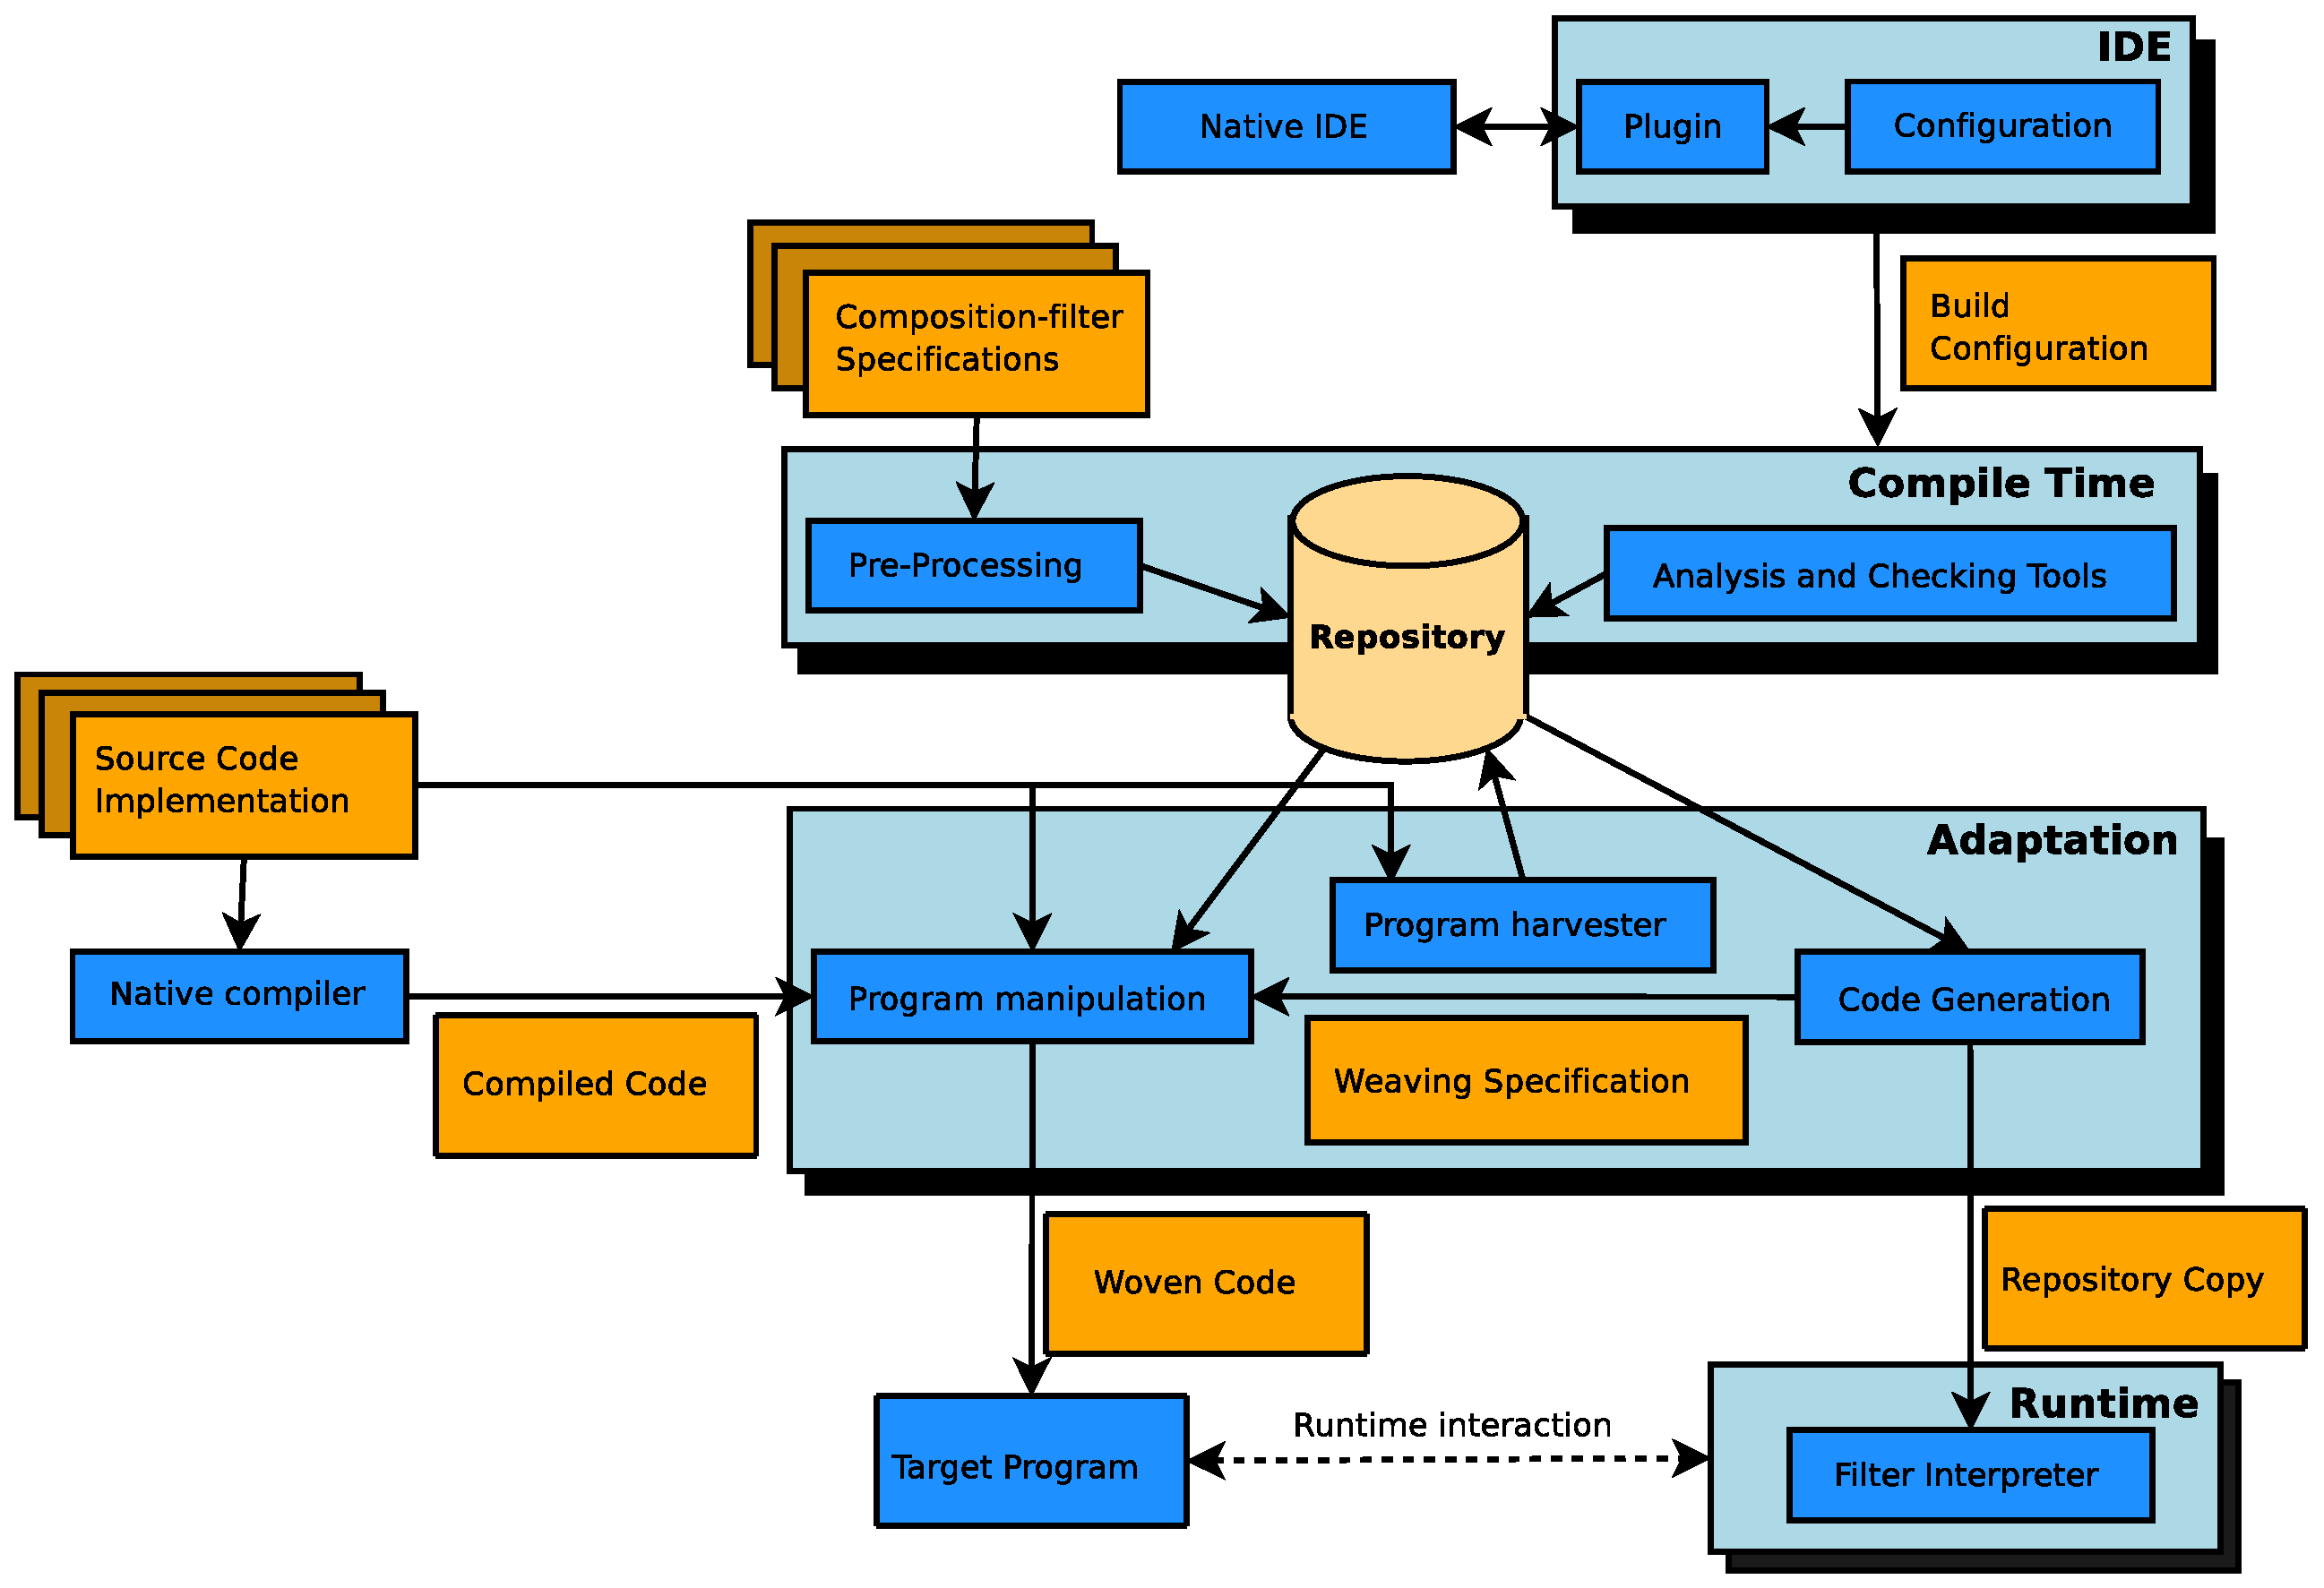
\includegraphics[style=halfheight]{Architecture05}
  \caption[Overview of the \Compose* architecture]{%
    Overview of the \Compose* architecture}
  \label{fig:ComposestarArchitecture}
\end{figure}
An overview of the \Compose* architecture is illustrated in \autoref{fig:ComposestarArchitecture}.
The \Compose* architecture can be divided in four layers~\cite{Nagy2006}: IDE, compile time, adaptation, and runtime. 

\subsection{Integrated Development Environment}
Some of the purposes of the Integrated Development Environment (IDE) layer are to interface with the native IDE and to create a build configuration.
In the build configuration it is specified which source files and settings are required to build a \Compose* application.
After creating the build configuration the compile time is started.

The creation of a build configuration can be done manually or by using a plug-in.
Examples of these plug-ins are the Visual Studio add-in for \Compose*[.NET] and the Eclipse plug-in for \Compose*[J] and \Compose*[C].

\subsection{Compile Time}
The compile time layer is platform independent and reasons about the correctness of the composition filter implementation with respect to the program which allows the target program to be build by the adaptation.

The compile time `pre-processes' the composition filter specifications by parsing the specification, resolving the references, and checking its consistency.
To provide an extensible architecture to facilitate this process a blackboard architecture is chosen.
This means that the compile time uses a general knowledgebase that is called the `repository'.
This knowledgebase contains the structure and metadata of the program which different modules can execute their activities on.
Examples of modules within analysis and validation are the three modules SANE, LOLA and FILTH.
These three modules are responsible for (some) of the analysis and validation of the super imposition and its selectors.

\subsection{Adaptation}
The adaptation layer consists of the program manipulation, harvester, and code generator.
These components connect the platform independent compile time to the target platform.
The harvester is responsible for gathering the structure and the annotations within the source program and adding this information to the knowledgebase.
The code generation generates a reduced copy of the knowledgebase and the weaving specification.
This weaving specification is then used by the weaver contained by the program manipulation to weave in the calls to the runtime into the target program.
The end result of the adaptation the target program which interfaces wit the runtime.

\subsection{Runtime}
The runtime layer is responsible for executing the concern code at the joinpoints.
It is activated at the joinpoints by function calls that are woven in by the weaver.
A reduced copy of the knowledgebase containing the necessary information for filter evaluation and execution is enclosed with the runtime.
When the function is filtered the filter is evaluated.
Depending on if the the condition part evaluates to true, and the matching part matches the accept or reject behavior of the filter is executed.
The runtime also facilitates the debugging of the composition filter implementations.

\section{Platforms}
The composition filters concept of \Compose* can be applied to any programming language, given that certain assumptions are met.
Currently, \Compose* supports three platforms: \dotNET, Java and C\@.
For each platform different tools are used for compilation and weaving.
They all share the same platform independent compile-time.

\Compose*[.NET] targets the \dotNET platform and is the oldest implementation of \Compose*.
Its weaver operates on CIL byte code.
\Compose*[.NET] is programming language independent as long as the programming language can be compiled to CIL code.
An add-in for Visual Studio is provided for ease of development.
\Compose*[J] targets the Java platform and provides a plug-in for integration with Eclipse.
\Compose*[C] contains support for the C programming language.
The implementation is different from the Java and \dotNET counterparts, because it does not have a run-time environment.
The filter logic is woven directly in the source code.
Because the language C is not based on objects, filters are woven on functions based on membership of sets of functions.
Like the Java platform, \Compose*[C] provides a plug-in for Eclipse.

%\section{Features explicit to \Compose*{}}
\section{Features Specific to \Compose*{}}
\label{section:FSTC}
The Composition Filters approach uses a restricted (pattern matching) language to define filters. This language makes it possible to reason about the semantics of the concern. 
\Compose* offers three features that use this possibility, which originate in more control and correctness over an application under construction. These features are:
\begin{description}[style=nextline,noitemsep]
\item [Ordering of filter modules] It is possible to specify how the superimposition of filter modules should be ordered. Ordering constraints can be specified in a fixed, conditional, or partial manner. A fixed ordering can be calculated exactly, whereas a conditional ordering is dependent on the result of filter execution and therefore evaluated at runtime. When there are multiple valid orderings of filtermodules on a join point, partial ordering constraints can be applied to reduce this number. These constraints can be declared in the concern definition;
\item [Filter consistency checking] When superimposition is applied, \Compose* is able to detect if the ordering and conjunction of filters creates a conflict. 
For example, imagine a set of filters where the first filter only evaluates method \emph{m} and another filter only evaluates methods \emph{a} and \emph{b}. 
In this case the latter filter is only reached with method \emph{m}; this is consequently rejected and as a result the superimposition may never be executed. There are different scenarios that lead to these kinds of problems, \eg conditions that exclude each other;
\item [Reason about semantic problems] When multiple pieces of advice are added to the same join point, \Compose* can reason about problems that may occur.
An example of such a conflict is the situation where a real-time filter is followed by a wait filter. Because the wait filter can wait indefinitely, the real-time property imposed by the real-time filter may be violated.
\end{description}
The above mentioned conflict analyzers all work on the assumption that the behavior of every filter is well-defined. This is not the case for the meta filter, its user-undefined, and therefore unpredictable, behavior poses a problem to the analysis tools. 

Furthermore, \Compose* is extended with features that enhance the usability. These features are briefly described below:
\begin{description}[style=nextline,noitemsep]
\item [Integrated Development Environment support] The \Compose* implementations all have a IDE plug-in; \Compose*[.NET] for Visual Studio, \Compose*[J] and \Compose*[C] for Eclipse;
\item [Debugging support] The debugger shows the flow of messages through the filters. It is possible to place breakpoints to view the state of the filters; 
\item [Incremental building process] When a project is build and not all the modules are changed, incremental building saves time.
\end{description}

Some language properties of \Compose* can also be seen as features, being:
\begin{description}[style=nextline,noitemsep]
\item [Language independent concerns] A \Compose* concern can be used for all the \Compose* platforms, because the composition filters approach is language independent;
\item [Reusable concerns] The concerns are easy to reuse, through the dynamic filter modules and the selector language;
\item [Expressive selector language] Program elements of an implementation language can be used to select a set of objects to superimpose on;
\item [Support for annotations] Using the selector, annotations can be woven at program elements. At the moment annotations can be used for superimposition. 
\end{description}




\chapter{Introduction to the \dotNET Framework}
\begin{flushright}
\textit{The best way to prepare [to be a programmer] is to write programs,}\\
\textit{and to study great programs that other people have written.}\\
\textit{In my case, I went to the garbage cans at the Computer Science Center}\\
\textit{and fished out listings of their operating system.}
\textit{William Henry Gates III}\\
\end{flushright}

\label{chp:dotnet_platform}

This chapter gives an introduction to the \dotNET Framework of Microsoft. First, the architecture of the \dotNET Framework is introduced. This section includes terms like the Common Language Runtime, the \dotNET Class Library, the Common Language Infrastructure and the Intermediate Language. These are discussed in more detail in the sections following the architecture.

\nomenclature{SOAP}{Simple Object Access Protocol}%
\nomenclature{WSDL}{Web Services Description Language}%
\section{Introduction}
Microsoft defines~\cite{Microsoft03-5} \dotNET as follows; ``\dotNET is the Microsoft Web services strategy to connect information, people, systems, and devices through software.''. There are different \dotNET technologies in various Microsoft products providing the capabilities to create solutions using web services. 
Web services are small, reusable applications that help computers from many different operating system platforms work together by exchanging messages. Based on industry standards like XML (Extensible Markup Language), SOAP (Simple Object Access Protocol), and WSDL (Web Services Description Language) they provide a platform and language independent way to communicate.

Microsoft products, such as Windows Server System (providing web services) or Office System (using web services) are some of the \dotNET technologies. The technology described in this chapter is the \dotNET Framework. Together with Visual Studio, an integrated development environment, they provide the developer tools to create programs for \dotNET. 

Many companies are largely dependent on the \dotNET Framework, but need or want to use AOP. Currently there is no direct support for this in the Framework. The \Compose*[.NET] project is addressing these needs with its implementation of the Composition Filters approach for the \dotNET Framework.

This specific \Compose* version for \dotNET has two main goals.
First, it combines the \dotNET Framework with AOP through Composition Filters.
Second, \Compose* offers superimposition in a language independent manner. The \dotNET Framework supports multiple languages and is, as such, suitable for this purpose.
Composition Filters are an extension of the object-oriented mechanism as offered by \dotNET, hence the implementation is not restricted to any specific object-oriented language.

\section{Architecture of the \dotNET Framework}
\label{sec:OverviewDotNetArchitecture}
\nomenclature{API}{Application Programming Interface}
The \dotNET Framework is Microsoft's platform for building, deploying, and running Web Services and applications. It is designed from scratch and has a consistent API providing support for component-based programs and Internet programming.
This new Application Programming Interface (API) has become an integral component of Windows. The \dotNET Framework was designed to fulfill the following objectives~\cite{Microsoft03-1}:

\begin{description}[noitemsep, style=nextline]
  \item[Consistency] Allow object code to be stored and executed locally, executed locally but Internet-distributed, or executed remotely and to make the developer experience consistent across a wide variety of types of applications, such as Windows-based applications and Web-based applications;
  \item[Operability] The ease of operation is enhanced by minimizing version conflicts and providing better software deployment support;
  \item[Security] All the code is executed safely, including code created by an unknown or semi-trusted third party;
  \item[Efficiency] The \dotNET Framework compiles applications to machine code before running thus eliminating the performance problems of scripted or interpreted environments;
  \item[Interoperability] Code based on the \dotNET Framework can integrate with other code because all communication is built on industry standards.
\end{description}

\begin{figure}
 \centering
 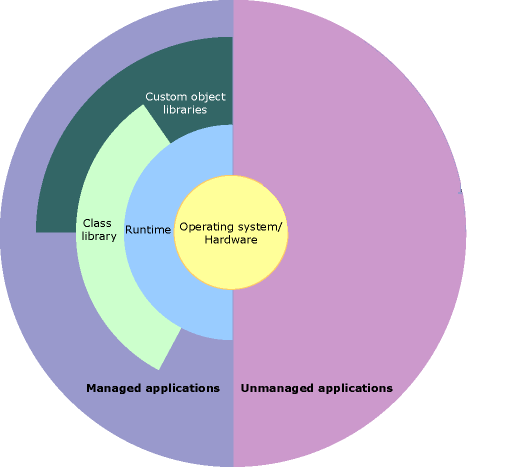
\includegraphics[style=thirdheight]{dotNET_context}
 \caption[Context of the \dotNET framework]{Context of the \dotNET Framework (Modified)~\cite{Microsoft03-1}}
 \label{fig:dotNET_context}
\end{figure}

\nomenclature{CLR}{Common Language Runtime}%
\nomenclature{CTS}{Common Type System}%
\nomenclature{CLS}{Common Language Specification}%
\nomenclature{FCL}{Framework Class Library}%
\nomenclature{CLI}{Common Language Infrastructure}%
The \dotNET Framework consists of two main components~\cite{Microsoft03-1}: the Common Language Runtime (CLR, simply called the \dotNET Runtime or Runtime for short) and the \dotNET Framework Class Library (FCL). 
The CLR is the foundation of the \dotNET Framework, executing the code and providing the core services such as memory management, thread management and exception handling. The CLR is described in more detail in \autoref{sec:clr}.
The class library, the other main component of the \dotNET Framework, is a comprehensive, object-oriented collection of reusable types that can be used to develop applications ranging from traditional command-line or graphical user interface (GUI) applications to applications such as Web Forms and XML Web services. \autoref{sec:fcl} describes the class libraries in more detail.

The code run by the runtime is in a format called Common Intermediate Language (CIL), further explained in~\autoref{sec:TheIntermediateLanguage}. The Common Language Infrastructure (CLI) is an open specification that describes the executable code and runtime environment that form the core of the Microsoft \dotNET Framework. \autoref{sec:cts} tells more about this specification.

\autoref{fig:dotNET_context} shows the relationship of the \dotNET Framework to other applications and to the complete system. The two parts, the class library and the runtime, are managed, \ie applications managed during execution. The operating system is in the core, managed and unmanaged applications operate on the hardware. The runtime can us other object libraries and the class library, but the other libraries can use the same class library them self.

Besides the Framework, Microsoft also provides a developer tool called the Visual Studio. This is an IDE with functionality across a wide range of areas allowing developers to build applications with decreased development time in comparison with developing applications using command line compilers.

\subsection{Version 2.0 of \dotNET}
\label{sec:Version2}
In November 2005, Microsoft released a successor of the \dotNET Framework. 
Major changes are the support for generics, the addition of nullable types, 64 bit support, improvements in the garbage collector, new security features and more network functionality.

Generics make it possible to declare and define classes, structures, interfaces, methods and delegates with unspecified or generic type parameters instead of specific types.
When the generic is used, the actual type is specified.
This allows for type-safety at compile-time.
Without generics, the use of casting or boxing and unboxing decreases performance.
By using a generic type, the risks and costs of these operations is reduced.

Nullable types allow a value type to have a normal value or a null value.
This null value can be useful for indicating that a variable has no defined value because the information is not currently available.

Besides changes in the Framework, there are also improvements in the four main Microsoft \dotNET programming languages (C\#, VB\dotNET, J\# and C++).
The language elements are now almost equal for all languages.
For instance, additions to the Visual Basic language are the support for unsigned values and new operators and additions to the C\# language include the ability to define anonymous methods thus eliminating the need to create a separate method.

A new Visual Studio 2005 edition was released to support the new Framework and functionalities to create various types of applications.

\section{Common Language Runtime}
\label{sec:clr}
The Common Language Runtime executes code and provides core services. These core services are memory management, thread execution, code safety verification and compilation. Apart from providing services, the CLR also enforces code access security and code robustness. 
Code access security is enforced by providing varying degrees of trust to components, based on a number of factors, \eg the origin of a component. 
This way, a managed component might or might not be able to perform sensitive functions, like file-access or registry-access. 
By implementing a strict type-and-code-verification infrastructure, called the Common Type System (CTS), the CLR enforces code robustness. Basically there are two types of code; 

\begin{description}[noitemsep,style=nextline]
\item[Managed]
Managed code is code, which has its memory handled and its types validated at execution by the CLR.
It has to conform to the Common Type Specification (CTS \autoref{sec:cts}).
If interoperability with components written in other languages is required, managed code has to conform to an even more strict set of specifications, the Common Language Specification (CLS).
The code is run by the CLR and is typically stored in an intermediate language format. This platform independent intermediate language is officially known as Common Intermediate Language (CIL \autoref{sec:TheIntermediateLanguage})~\cite{Watkins00}.
\item[Unmanaged]
Unmanaged code is not managed by the CLR. It is stored in the native machine language and is not run by the runtime but directly by the processor.
\end{description}
\nomenclature{JIT}{Just-in-time}

All language compilers (targeting the CLR) generate managed code (CIL) that conforms to the CTS. 

At runtime, the CLR is responsible for generating platform specific code, which can actually be executed on the target platform.
Compiling from CIL to the native machine language of the platform is executed by the just-in-time (JIT) compiler. Because of this language independent layer it allows the development of CLRs for any platform, creating a true interoperability infrastructure~\cite{Watkins00}.
The \dotNET Runtime from Microsoft is actually a specific CLR implementation for the Windows platform.
\nomenclature{PDA}{Personal Digital Assistant}
Microsoft has released the \emph{\dotNET Compact Framework} especially for devices such as personal digital assistants (PDAs) and mobile phones.
The \dotNET Compact Framework contains a subset of the normal \dotNET Framework and allows \dotNET developer to write mobile applications. Components can be exchanged and web services can be used so an easier interoperability between mobile devices and workstations/servers can be implemented~\cite{Microsoft03-3}.

At the time of writing, the \dotNET Framework is the only advanced Common Language Infrastructure (CLI) implementation available.
A shared-source\footnote{Only non-commercial purposes are allowed.} implementation of the CLI for research and teaching purposes was made available by Microsoft in 2002 under the name Rotor~\cite{Stutz02}. In 2006 Microsoft released an updated version of Rotor for the \dotNET platform version two.
Also Ximian is working on an open source implementation of the CLI under the name Mono\footnote{\url{http://www.go-mono.com/}}, targeting both Unix/Linux and Windows platforms.
Another, somewhat different approach, is called Plataforma.NET\footnote{\url{http://personals.ac.upc.edu/enric/PFC/Plataforma.NET/p.net.html}} and aims to be a hardware implementation of the CLR, so that CIL code can be run natively.

\subsection{Java VM vs \dotNET CLR}
There are many similarities between Java and \dotNET technology. This is not strange, because both products serve the same market.

\nomenclature{JVM}{Java Virtual Machine}
Both Java and \dotNET are based on a runtime environment and an extensive development framework.
These development frameworks provide largely the same functionality for both Java and \dotNET.
The most obvious difference between them is lack of language independence in Java.
While Java's strategy is `One language for all platforms' the \dotNET philosophy is `All languages on one platform'.
However these philosophies are not as strict as they seem.
As noted in \autoref{sec:fcl} there is no technical obstacle for other platforms to implement the \dotNET Framework.
There are compilers for non-Java languages like Jython (Python)~\cite{Jython03} and WebADA~\cite{Ada96} available for the JVM.
Thus, the JVM in its current state, has difficulties supporting such a vast array of languages as the CLR.
However, the multiple language support in \dotNET is not optimal and has been the target of some criticism.

Although the JVM and the CLR provide the same basic features they differ in some ways.
While both CLR and the modern JVM use JIT (Just In Time) compilation the CLR can directly access native functions.
This means that with the JVM an indirect mapping is needed to interface directly with the operating system.
\section{Common Language Infrastructure}
\label{sec:cts}
The entire CLI has been documented, standardized and approved~\cite{Ecma-335} by the European association for standardizing information and communication systems, Ecma International\footnote{An European industry association founded in 1961 and dedicated to the standardization of Information and Communication Technology (ICT) Systems.
Their website can be found at \url{http://www.ecma-international.org/}.}.
Benefits of this CLI for developers and end-users are:

\begin{itemize}[noitemsep]
  \item Most high level programming languages can easily be mapped onto the Common Type System (CTS);
  \item The same application will run on different CLI implementations;
  \item Cross-programming language integration, if the code strictly conforms to the Common Language Specification (CLS);
  \item Different CLI implementations can communicate with each other, providing applications with easy cross-platform communication means.
\end{itemize}

This interoperability and portability is, for instance, achieved by using a standardized meta data and intermediate language (CIL) scheme as the storage and distribution format for applications.
In other words, (almost) any programming language can be mapped to CIL, which in turn can be mapped to any native machine language.

The Common Language Specification is a subset of the Common Type System, and defines the basic set of language features that all \dotNET languages should adhere to.
In this way, the CLS helps to enhance and ensure language interoperability by defining a set of features that are available in a wide variety of languages.
The CLS was designed to include all the language constructs that are commonly needed by developers 
(\eg naming conventions, common primitive types), but no more than most languages are able to support~\cite{Microsoft03-2}.
\autoref{fig:Common_Type_System} shows the relationships between the CTS, the CLS, and the types available in C++ and C\#.
\begin{figure}
 \centering
 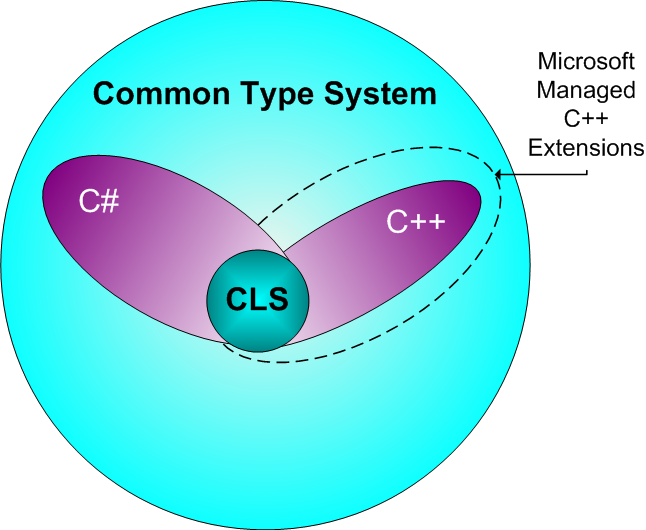
\includegraphics[style=fourthheight]{Common_Type_System}
 \caption{Relationships in the CTS}
 \label{fig:Common_Type_System}
\end{figure}
In this way the standardized CLI provides, in theory\footnote{Unfortunately Microsoft did not submit all the framework classes for approval and at the time of writing only the \dotNET Framework implementation is stable.}, a true cross-language and cross-platform development and runtime environment.

To attract a large number of developers for the \dotNET Framework, Microsoft has released CIL compilers for C++, C\#, J\#, and VB.NET.
In addition, third-party vendors and open-source projects also released compilers targeting the \dotNET Framework, such as Delphi.NET, Perl.NET, IronPython, and Eiffel.NET.
These programming languages cover a wide-range of different programming paradigms, such as classic imperative, object-oriented, scripting, and declarative languages. This wide coverage demonstrates the power of the standardized CLI.

\begin{figure}
 \centering
 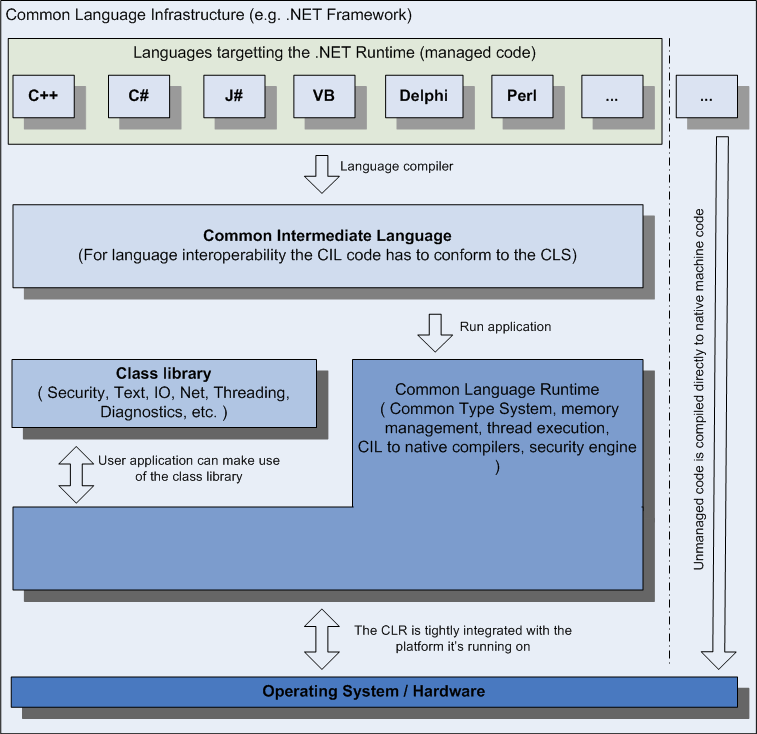
\includegraphics[style=halfheight]{Common_Language_Infrastructure}
 \caption[Main components of the CLI and their relationships]{%
    Main components of the CLI and their relationships.
    The right hand side of the figure shows the difference between managed code and unmanaged code.}
 \label{fig:Common_Language_Infrastructure}
\end{figure}

\autoref{fig:Common_Language_Infrastructure} shows the relationships between all the main components of the CLI.
The top of the figure shows the different programming languages with compiler support for the CLI. Because the compiled code is stored and distributed in the Common Intermediate Language format, the code can run on any CLR. For cross-language usage this code has to comply with the CLS.
Any application can use the class library (the FCL) for common and specialized programming tasks. 
\section{Framework Class Library}
\label{sec:fcl}
The \dotNET Framework class library is a comprehensive collection of object-oriented reusable types for the CLR. 
This library is the foundation on which all the \dotNET applications are built.
It is object oriented and provides integration of third-party components with the classes in the \dotNET Framework.
Developers can use components provided by the \dotNET Framework, other developers and their own components.
\nomenclature{GUI}{Graphical User Interface}%
\nomenclature{XML}{eXtensible Markup Language}%
A wide range of common programming tasks (\eg string management, data collection, reflection, graphics, database connectivity or file access) can be accomplished easily by using the class library.
Also, a great number of specialized development tasks are extensively supported, like:
\begin{itemize}[noitemsep]
  \item Console applications;
  \item Windows GUI applications (Windows Forms);
  \item Web applications (Web Forms);
  \item XML Web services;
  \item Windows services.
\end{itemize}
All the types in this framework are CLS compliant and can therefore be used from any programming language whose compiler conforms to the Common Language Specification (CLS).
\section{Common Intermediate Language}
\label{sec:TheIntermediateLanguage}
The Common Intermediate Language (CIL) has already been mentioned briefly in the sections before, but this section will describe the IL in more detail.
All the languages targeting the \dotNET Framework compile to this CIL (see \autoref{fig:Overview_of_the_Common_Language_Infrastructure}).

\begin{figure}[htbp]
  \centering
  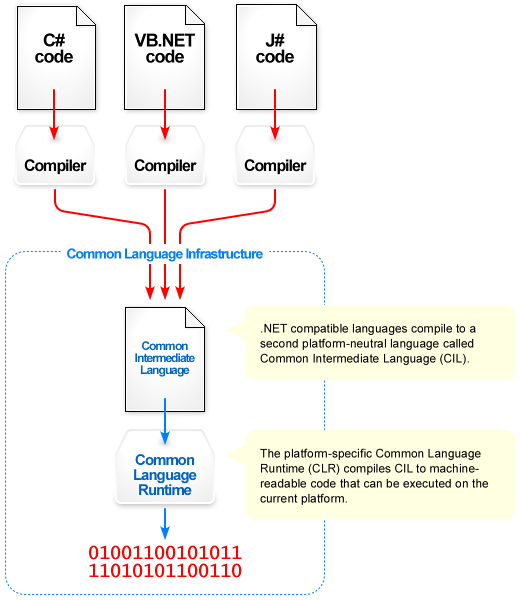
\includegraphics[style=halfheight]{Overview_of_the_Common_Language_Infrastructure}
  \caption{From source code to machine code}
  \label{fig:Overview_of_the_Common_Language_Infrastructure}
\end{figure}

A \dotNET compiler generates a \emph{managed module} which is an executable designed to be run by the CLR~\cite{Prosise2002}.
There are four main elements inside a managed module:

\begin{itemize}[noitemsep]
  \item A Windows Portable Executable (PE) file header;
  \item A CLR header containing important information about the module, such as the location of its CIL and metadata;
  \item Metadata describing everything inside the module and its external dependencies;
  \item The CIL instructions generated from the source code.
\end{itemize}

The Portable Executable file header allows the user to start the executable.
This small piece of code will initiate the just-in-time compiler which compiles the CIL instructions to native code when needed, while using the metadata for extra information about the program.
This native code is machine dependent while the original IL code is still machine independent.
This way the same IL code can be JIT-compiled and executed on any supported architecture.
The CLR cannot use the managed module directly but needs an assembly. 

An assembly is the fundamental unit of security, versioning, and deployment in the \dotNET Framework and is a collection of one or more files grouped together to form a logical unit~\cite{Prosise2002}.
Besides managed modules inside an assembly, it is also possible to include resources like images or text.
A manifest file is contained in the assembly describing not only the name, culture and version of the assembly but also the references to other files in the assembly and security requests.

\nomenclature{OpCode}{Operation Code}%
The CIL is an object oriented assembly language with around 100 different instructions called OpCodes.
It is stack-based, meaning objects are placed on an evaluation stack before the execution of an operation, and when applicable, the result can be found on the  stack after the operation.
For instance, when adding two numbers, first those numbers have to be placed onto the stack, second the add operation is called and finally the result can be retrieved from the stack.

\begin{lstlisting}[language=CIL,style=listing,caption={Adding example in IL code},label={lst:ilexample}]
.assembly AddExample {}

.method static public void main() il managed
{
  .entrypoint           // entry point of the application
  .maxstack 2

  ldc.i4 3              // Place a 32-bit (i4) 3 onto the stack
  ldc.i4 7              // Place a 32-bit (i4) 7 onto the stack
	
  add                   // Add the two and 
	                      // leave the sum on the stack
  
  // Call static System.Console.Writeline function
  // (function pops integer from the stack)
  call void [mscorlib]System.Console::WriteLine(int32)

  ret
}
\end{lstlisting}

To illustrate how to create a \dotNET program in IL code we use the previous example of adding two numbers and show the result.
In \autoref{lst:ilexample} a new assembly is created with the name \lstinline|AddExample|.
In this assembly a function \lstinline|main| is declared as the starting point (\lstinline|entrypoint|) of this assembly.
The \lstinline|maxstack| command indicates there can be a maximum of two objects on the stack and this is enough for the example method.
Next, the values 3 and 7 are placed onto the stack. The \lstinline|add| operation is called and the results stays on the stack.
The method \lstinline|WriteLine| from the \dotNET Framework Class Library is called.
This method resides inside the \lstinline|Console| class placed in the \lstinline|System| assembly.
It expects one parameter with a \lstinline|int32| as its type that will be retrieved from the stack.
The \lstinline|call| operation will transfer the control flow to this method passing along the parameters as objects on the stack.
The \lstinline|WriteLine| method does not return a value.
The \lstinline|ret| operation returns the control flow from the main method to the calling method, in this case the runtime.
This will exit the program.

To be able to run this example, we need to compile the IL code to bytecode where each OpCode is represented as one byte.
To compile this example, save it as a text file and run the \emph{ILASM} compiler with as parameter the filename.
This will produce an executable runnable on all the platforms where the \dotNET Framework is installed.

This example was written directly in IL code, but we could have used a higher level language such as C\# or VB\dotNET. For instance, the same example in C\# code is shown in~\autoref{lst:CSharpAddExample} and the VB\dotNET version is listed in~\autoref{lst:VBAddExample}. When this code is compiled to IL, it will look like the code in~\autoref{lst:ilexample}.

\begin{lstlisting}[language={[Sharp]C},style=listing,caption={Adding example in the C\# language},label={lst:CSharpAddExample}]
public static void main()
{
      Console.WriteLine((int) (3 + 7));
} 
\end{lstlisting} 

\begin{lstlisting}[language={[Visual]{Basic}},style=listing,caption={Adding example in the VB\dotNET language},label={lst:VBAddExample}]
Public Shared Sub main()
      Console.WriteLine(CType((3 + 7), Integer))
End Sub
\end{lstlisting} 

 



% Backmatter
\bibliography{references/general,references/dotnet,references/composestar,references/aosd-bibliography}

\end{document}

